\chapter{Landasan Teori}

\section {Arsitektur Sistem Pakar}
Sistem pakar (Expert System) adalah sistem informasi berbasi komputer yang menggunakan pengetahuan ahli atau pakar untuk mencapai kinerja pengambilan keputusan tingat tinggi dalam domain masalah yang ditentukan menurut Turban \cite{turban}. Berikut Gambar \ref{fig:komponen} memperlihatkan arsitektur komponen pembangun sistem pakar: 

\begin{figure}[h]	
	{\centering {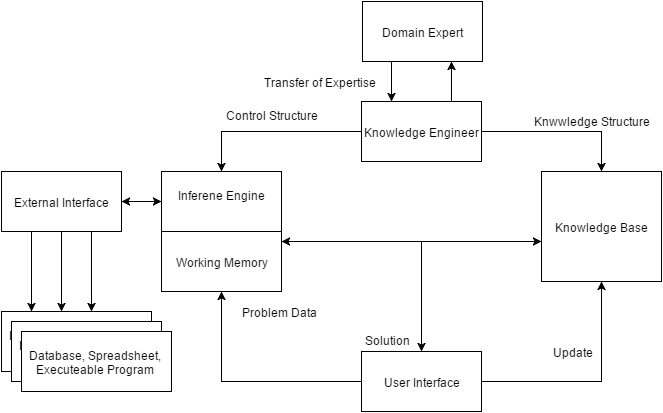
\includegraphics[scale=0.8]{gambarArsitektur.png}}\par}
	\caption{Komponen Sistem Pakar \cite{mca2015}}
	\label{fig:komponen}
\end{figure}
Penjelasan komponen penyusun dari sistem pakar sebagai berikut:

\begin{itemize}
	\item User Interface\\
	Tampilan antarmuka sebagai media komunikasi antara pengguna dengan sistem pakar.
	\item Knowledge Base\\
	Basis pengetahuan berisi pengetahuan yang relevan untuk sistem memahami, merumuskan dan memecahkan masalah. Terdiri dari dua elemen dasar yaitu fakta (facts) dan aturan (rules). Fakta menggambarkan karakteristik situasi masalah dan teori pada bidang masalah. Aturan mewakili pengetahuan ahli untuk memecahkan masalah tertentu dalam domain.
	\item Knowledge Acquisition\\
	Akuisisi pengetahuan pemecahan masalah dari pakar atau sumber pengetahuan terdokumentasi lain untuk program komputer. Potensi sumber pengetahuan bisa berupa manusia, buku teks, dokumen multimedia, database, dan laporan penelitian.
	\item Inference Engine \\
	Merupakan otak dari sistem pakar. Komponen ini menyediakan suatu metode untuk penalaran (reasoning) infromasi yang terdapat dalam knowledge base dan workplace untuk merumuskan kesimpulan.
	\item 	Workplace \\
	Sebagai tempat penyimpanan data masalah berupa hasil sementara, hipotesis dan keputusan yang sedang dikerjakan. 
	\item Explanation Subsystem \\
	Komponen tambahan yang meningkatkan kemampuan sistem pakar dengan menjelaskan kelakuan sistem pakar secara interaktif melalui jawaban pertanyaan.
	\item Knowledge Refining System \\
	Orang yang ahli di bidang tertentu dapat melakukan analisis dan peningkatan performa penafsiran miliknya. Begitu juga sistem pakar membutuhkan evaluasi untuk meningkatkan hasil yang lebih akurat melalui knowledge base serta kemampuan reasoning yang lebih efektif. 	
\end{itemize}

\section{\textit{Forward Chaining}}
Merupakan salah satu metode inferensi yang menghasilkan solusi dengan melakukan penalaran terhadap suatu masalah. Dikenal juga dengan data-driven karena inferensi dimulai dengan informasi yang tersedia kemudian baru menghasilkan konklusi. Pola pendekatan penalaran forward chaining adalah IF (informasi) THEN (konklusi). Pelacakan kedepan dilakukan dari sekumpulan fakta dan mencari kaidah yang cocok hingga menuju kesimpulan. Berikut Algoritma \ref{forwardChaining} merupakan contoh dari proses forward chaining dalam menghasilkan konklusi dari aturan produksi: 
\begin{algorithm}
	\caption{Forward chaining}
	\label{forwardChaining}
	\begin{algorithmic}[1]
		\If {$(Pasien$ $Hamil)$ AND $(kontraksi)$  AND $(premature)$}
		\State $UGD Rumah$$ Bersalin$
		\EndIf
	\end{algorithmic}
\end{algorithm}

Berikut gambar \ref{fig:inferensi} tentang ilustrasi dari proses yang terjadi pada mesin inferensi:

\begin{figure}[h]	
	{\centering {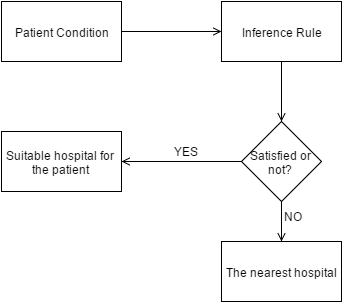
\includegraphics[scale=1]{mesinInferensi.png}}\par}
	\caption{Proses Mesin Inferensi}
	\label{fig:inferensi}
\end{figure}

Penjelasan dari proses mesin inferensi pada Gambar \ref{fig:inferensi} adalah dengan input berupa kondisi pasien. Misal pasien mengalami kelahiran premature. Dengan aturan inferensi dilakukan pengecekan dari knowledge base terhadap kecocokan rumah sakit. Mesin inferensi akan memeriksa aturan produksi terhadap UGD rumah sakit A, UGD rumah sakit B dan seterusnya. Berdasarkan kondisi pasien yang digunakan sebagai contoh maka UGD yang cocok memiliki factor waktu tempuh terdekat, terdapat dokter jaga, terdapat dokter Gynecology, tersedia ruang bersalin yang sedang kosong.

\section{Algoritma Rete}
Charles R.Forgy \cite{charles1982} mengembangkan algoritma Rete yang dikenal efisien dalam menyelesaikan berbagai permasalahan pattern matching. Merupakan solusi dari beberapa permasalahan di sistem pakar dimana jika knowledge base terdiri dari banyak rules akan menurunkan performansi. Ide utama dari algoritma rete adalah dengan melakukan komputasi himpunan rules secara instantiation incremental, berdasarkan dua pendekatan:
\begin{enumerate}
	\item Memorisation:\\ Untuk setiap siklus ke siklus selanjutnya tidak terjadi perubahan yang berarti terhadap himpunan rules. Sehingga hanya dilakukan komputasi di perubahan yang terjadi, sedangkan beberapa bagian rules tetap dipertahankan. Tidak perlu melakukan komputasi rules menyeluruh untuk tiap siklus. 
	\item Sharing:\\  Beberapa rules digunakan sebagai kondisi sama yang sering terjadi, sehingga seluruh rules difaktorkan kedalam kondisi yang terdapat mirip.
\end{enumerate}	
Implementasi algoritma Rete yaitu dengan membuat hubungan antar node yang membentuk suatu jaringan. Hubungan antar node dirancang agar bisa menghemat proses komputasi dari suatu siklus ke siklus selanjutnya. Komputasi ulang perubahan hanya untuk fakta-fakta yang akan dimodifikasi. Sebagai contoh missal diketahui sebuah rule sebagai berikut: If age fewer than 60 or age fewer than 5 or income fewer than 36000 then concession = 50/100. 
Maka jaringan Rete yang tersebut akan seperti di Gambar \ref{fig:rete} dibawah ini:
\begin{figure}[h]	
	{\centering {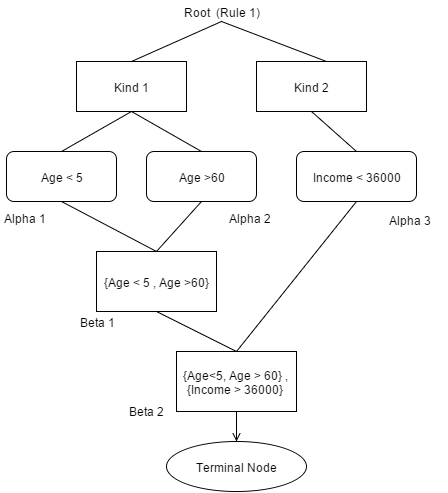
\includegraphics[scale=0.8]{jaringanRete.png}}\par}
	\caption{Contoh Jaringan terbentuk  dari algoritma Rete}
	\label{fig:rete}
\end{figure}

Penjelasan dari jaringan yang terbentuk oleh algoritma Rete pada Gambar \ref{fig:rete} adalah sebagai berikut :
\begin{enumerate}
	\item Alpha Network\\
	Berfungsi untuk memilih individu working memory element (WME) berdasarkan uji kondisional sederhana untuk membandingkan node WME yang memiliki kesamaan atribut. Percabangan mungkin terjadi pada Alpha node untuk meminimalkan redundansi.
	\item Beta Network\\
	Merupakan gabungan dari WME dan melakukan pemrosesan token. Token adalah unit penyimpanan yang berada di memori dan unit pertukaran antar memori dengan node. Setiap Beta node dapat menghasilkan token baru untuk menahan daftar WME yang merepresentasikan kecocokan partial. WME yang mencapai ujung cabang dari Beta Node merepresentasikan tahap lengkap kecocokan untuk satu produksi. Kemudian proses selanjutnya dikirim ke terminal node.
	\item Conflict Resolution\\
	Pada setiap satu siklus match-resolve-act, mesin inferensi akan menemukan semua kemungkinan kecocokan untuk fakta yang sedang diolah di working memory. Setelah semua kecocokan ditemukan, aturan produksi yang berhubungan telah diaktifkan dalam agenda. Mesin inferensi akan menentukan aturan produksi yang tereksekusi.  
\end{enumerate}

\section{Related Works}
Penelitian terkait untuk kasus ini dilakukan Zhen \cite{zhen2014} dalam penelitiannya membangun  decision rule  untuk  penjadwalan mobil ambulans. Dalam penelitan Zhen \cite{zhen2014} memperhitungan rata-rata response time dan data stokastik kondisi lalu lintas, waktu tempuh sehingga korban gawat darurat dapat dicapai dalam waktu yang efisien. Hasilnya permintaan mobil ambulans dapat dipenuhi tepat waktu sesuai rule yang dibangun. Bowen \cite{james1998} dalam penelitiannya menggunakan sistem keputusan untuk relokasi persebaran ambulan di daerah perkotaaan dengan harapan meningkatkan kesiapan ketika terjadi kejadian gawat darurat.  Hasilnya berupa distribusi mobil ambulans yang mampu melayani permintaan di satu area secara menyeluruh. Penelitian \cite{zhen2014} dan Bowen \cite{james1998} berpusat pada bagaimana meningkatkan kinerja unit ambulan sebagai transportasi ketika terjadi kejadian gawat darurat. Namun, dalam rangka memberikan pertolongan terhadap korban gawat darurat dapat tidak hanya dibutuhkan peningkatan pelayanan mobil ambulans tetapi juga ketepatan pemilihan unit gawat darurat tujuan dengan memperhatikan sudut pandang korban dan sumber daya UGD apapun mode transportasinya.   \par
Weng dan Kuo \cite{weng2009} dalam penelitiannya membangun sistem informasi pakar gawat darurat untuk daerah dengan sumber daya medis yang kurang. Faktor yang digunakan dalma pemilihan UGD adalah kondisi pasien, jarak dari lokasi kejadian gawat darurat ke UGD tujuan,ketersediaan dokter jaga, ketersediaan ruang operasi, ketersediaan ruang ICU, ketersediaan ruang inap. Dalam penelitian tersebut dikembangkan kaidah pemilihan unit gawat darurat berdasar kondisi korban. Kaidah yang dibangun memungkinkan sistem menampilkan rumah sakit yang cocok untuk korban pada waktu kejadian gawat darurat menggunakan pola runut maju (Forward Chaining). Priyandari \cite{priyandari2011} menggunakan model kaidah pemilihan UGD dari penelitian Weng dan Kuo tetapi mengganti kriteria jarak dengan estimasi waktu tempuh untuk mengatasi arus lalulintas perkotaan yang padat. Mesin inferensi yang digunakan sama yaitu forward chaining.
\par
Dalam penelitian tugas akhir ini penulis mempertimbangkan penggunaan faktor pemilihan UGD yang dikembangkan pada penelitian Priyandari \cite{priyandari2011} dan dilakukan studi lebih lanjut model kaidah pemilihan UGD hasil dari penelitian Weng dan Kuo \cite{weng2009} untuk disesuaikan dengan studi kasus pada tugas akhir ini. Sistem yang akan dibangun berupa sistem pakar pemilihan UGD untuk wilayah kota Bandung. Algoritma yang akan diterapkan pada inference engine adalah algoritma Rete. 

